\chapter{Oscilloscope Drivers}
\label{sec:drivers}

\section{Agilent}

Agilent devices support a similar similar SCPI command set across most device families.

Please see the table below for details of current hardware support:

\begin{tabularx}{16cm}{lllX}
\thickhline
\textbf{Device Family} & \textbf{Driver} & \textbf{Transport} & \textbf{Notes} \\
\thickhline
DSO5000 series & agilent & lan & Not recently tested, but should work.\\
\thinhline
DSO6000 \& MSO6000 series & agilent & lan &  Working. No support for digital channels yet.\\
\thinhline
DSO7000 \& MSO7000 series & agilent & lan & Untested, but should work. No support for digital channels yet.\\
\thinhline
MSOX-2000 series & agilent & lan \\
\thinhline
MSOX-3000 series & agilent & lan \\
\thickhline
\end{tabularx}

\subsection{agilent}

\subsubsection{Typical Performance (MSO6034A, LAN)}

Interestingly, performance sometimes gets better with more channels or deeper memory. Not sure why.

\begin{tabularx}{16cm}{llX}
\thickhline
\textbf{Channels} & \textbf{Memory depth} & \textbf{WFM/s}\\
\thickhline
1 & 1K & 66 \\
\thinhline
4 & 1K & 33 \\
\thinhline
4 & 4K & 33 \\
\thinhline
1 & 40K & 33 \\
\thinhline
1 & 4K & 22 \\
\thinhline
1 & 20K & 22 \\
\thinhline
4 & 20K & 22 \\
\thinhline
1 & 100K & 22 \\
\thinhline
4 & 10K & 17 \\
\thinhline
4 & 40K & 12 \\
\thinhline
1 & 200K & 11 \\
\thinhline
1 & 400K & 8 \\
\thinhline
4 & 100K & 6.5 \\
\thinhline
4 & 200K & 4 \\
\thinhline
1 & 1M & 3.7 \\
\thinhline
4 & 400K & 2.3 \\
\thinhline
1 & 1M & 1 \\
\thinhline
4 & 1M & 1 \\
\thinhline
4 & 4M & 0.2 \\
\thickhline
\end{tabularx}

\subsubsection{Typical Performance (MSOX3104T, LAN)}

\begin{tabularx}{16cm}{llX}
\thickhline
\textbf{Channels} & \textbf{Memory depth} & \textbf{WFM/s}\\
\thickhline
1 & 2.5K & 3.3 \\
\thinhline
4 & 2.5K & 2.5 \\
\thinhline
1 & 2.5M & 1.0 \\
\thinhline
4 & 2.0M & 0.5 \\
\thickhline
\end{tabularx}

\section{Antikernel Labs}

\begin{tabularx}{16cm}{llX}
\thickhline
\textbf{Device Family} & \textbf{Driver} & \textbf{Notes} \\
\thickhline
Internal Logic Analyzer IP & akila & \\
\thickhline
BLONDEL Oscilloscope Prototype & aklabs & \\
\thickhline
\end{tabularx}

\subsection{akila}

This driver uses a raw binary protocol, not SCPI.

Under-development internal logic analyzer analyzer core for FPGA design debug. The ILA uses a UART interface to a host
system. Since there's no UART support in scopehal yet, socat must be used to bridge the UART to a TCP socket using
the ``lan" transport.

\subsection{aklabs}

This driver uses two TCP sockets. Port 5025 is used for SCPI control plane traffic, and port 50101 is used for waveform
data using a raw binary protocol.

\section{Demo}

The ``demo" driver is a simulation-only driver for development and training purposes, and does not connect to real
hardware.

It ignores any transport provided, and is normally used with the ``null" transport.

The demo instrument is intended to illustrate the usage of glscopeclient for various types of analysis and to aid in
automated testing on computers which do not have a connection to a real oscilloscope, and is not intended to accurately
model the response or characteristics of real world scope frontends or signals.

It supports memory depths of 10K, 100K, 1M, and 10M points per waveform at rates of 1, 5, 10, 25, 50, and 100 Gsps.
Four test signals are provided, each with 10 mV of Gaussian noise and a 5 GHz low-pass filter added (although this can
be disabled under the channel properties)

Test signals:
\begin{itemize}
\item 1.000 GHz tone
\item 1.000 GHz tone mixed with a second tone, which sweeps from 1.100 to 1.500 GHz
\item 10.3125 Gbps PRBS-31
\item 1.25 Gbps repeating two 8B/10B symbols (K28.5 D16.2)
\end{itemize}

\begin{tabularx}{16cm}{lllX}
\thickhline
\textbf{Device Family} & \textbf{Driver} & \textbf{Transport} & \textbf{Notes} \\
\thickhline
Simulator & demo & null & \\
\thickhline
\end{tabularx}

\section{Digilent}

Digilent oscilloscopes using the WaveForms SDK are all supported using the ``digilent" driver in libscopehal. This
driver connects using the ``twinlan" transport to a \href{https://github.com/azonenberg/scopehal-waveforms-bridge}
{socket server} which links against the Digilent WaveForms SDK. This provides network transparency, and allows the
Digilent bridge server to be packaged separately for distribution and only installed by users who require it.

As of 2022-03-09, analog input channels on the Analog Discovery Pro and Analog Discovery 2 have been tested and are
functional, however only basic edge triggering is implemented so far. Analog inputs on other devices likely work,
however only these two have been tested to date.

Analog outputs, digital inputs, and digital outputs are currently unimplemented, but are planned to be added in the
future.

\subsection{digilent}

\begin{tabularx}{16cm}{lllX}
\thickhline
\textbf{Device Family} & \textbf{Driver} & \textbf{Transport} & \textbf{Notes} \\
\thickhline
Electronics Explorer & digilent & twinlan & Not tested, but probably works\\
\thinhline
Analog Discovery & digilent & twinlan & Not tested, but probably works\\
\thinhline
Analog Discovery 2 & digilent & twinlan & No digital channel support \newline No analog output support\\
\thinhline
Analog Discovery Pro & digilent & twinlan & No digital channel support \newline No analog output support \\
\thinhline
Digital Discovery & digilent & twinlan & No digital channel support,\newline so pretty useless for now\\
\thickhline
\end{tabularx}

\subsubsection{Typical Performance (ADP3450, USB -> LAN)}

\begin{tabularx}{16cm}{llX}
\thickhline
\textbf{Channels} & \textbf{Memory depth} & \textbf{WFM/s}\\
\thickhline
4 & 64K & 25.8 \\
\thinhline
2 & 64K & 32.3 \\
\thinhline
1 & 64K & 33.0 \\
\thickhline
\end{tabularx}

\section{DreamSource Lab}

DreamSourceLabs oscilloscopes and logic analyzers supported in their fork of sigrok (``libsigrok4DSL'' distributed as part of
their ``DSView'' software package) are supported through the ``dslabs'' driver in libscopehal. This driver connects using
the ``twinlan'' transport to a \href{https://github.com/glscopeclient/scopehal-sigrok-bridge}{socket server} which links
against libsigrok4DSL. This provides network transparency, and allows the DSLabs bridge server to be packaged separately for
distribution and only installed by users who require it.

As of 2022-03-22, a DSCope U3P100 and a DSLogic U3Pro16has been tested and works adequately. Other products may work
also, but are untested.

On DSCope: Only edge triggers are supported. `Any' edge is not supported. ``Ch0 \&\& Ch1'' and ``Ch0 || Ch1'' trigger modes
are not supported.

On DSLogic: Only edge triggers are supported. All edges are supported. There is currently no way to configure a trigger on more
than one channel. Serial / multi-stage triggers are not supported.

Known issues pending fixes/refactoring:
\begin{itemize}
	\item Interleaved sample rates are not correctly reported in the timebase dialog (but are in the waveform display)
	\item Trigger position is quantized to multiples of 1\% of total capture
	\item Non-localhost performance, and responsiveness in general may suffer as a result of hacky flow control on waveform capture
	\item DSLogic depth configuration is confusing and performance could be improved (currently only buffered more is supported)
	\item DSLogic devices trigger even if pre-trigger buffer has not been filled, leading to a small pre-trigger waveform in some cases
\end{itemize}

\subsection{dslabs}

\begin{tabularx}{16cm}{lllX}
\thickhline
\textbf{Family / Device} & \textbf{Driver} & \textbf{Transport} & \textbf{Notes} \\
\thickhline
DSCope U3P100 & dslabs & twinlan & Tested, works\\
\thinhline
DSLogic U3P16 & dslabs & twinlan & Tested, works\\
\thinhline
DSCope (others) & dslabs & twinlan & Not tested, but probably works\\
\thinhline
DSLogic (others) & dslabs & twinlan & Not tested, but probably works\\
\thickhline
\end{tabularx}

\subsubsection{Typical DSCope Performance (DSCope U3P100, USB3, localhost)}

\begin{tabularx}{16cm}{lllXX}
\thickhline
\textbf{Channels} & \textbf{Memory depth} & \textbf{Sample Rate} & \textbf{WFM/s} & \textbf{UI-unconstrained WFM/s}\\
\thickhline
2 & 1M & 100MS/s & 14 & 50\\
\thinhline
2 & 5M & 500MS/s & 4.5 & 14\\
\thinhline
1 & 5M & 1GS/s & 8.3 & 32\\
\thickhline
\end{tabularx}

\subsubsection{Typical DSLogic Performance (DSLogic U3Pro16, USB3, localhost)}

\begin{tabularx}{16cm}{lllXX}
\thickhline
\textbf{Channels} & \textbf{Memory depth} & \textbf{Sample Rate} & \textbf{WFM/s} & \textbf{UI-unconstrained WFM/s}\\
\thickhline
16 & 500k & 100MS/s & 16 & 44\\
\thinhline
16 & 500k & 500MS/s & 16 & 55\\
\thickhline
\end{tabularx}

\section{Enjoy Digital}
TODO (\issue{scopehal}{79})

\section{Hantek}
TODO (\issue{scopehal}{26})

\section{Keysight}

Keysight devices support a similar similar SCPI command set across most device families. Many Keysight devices were
previously sold under the Agilent brand and use the same SCPI command set, so they are supported by the ``agilent"
driver.

Please see the table below for details of current hardware support:

\subsection{agilent}

\begin{tabularx}{16cm}{llX}
\thickhline
\textbf{Device Family} & \textbf{Driver} & \textbf{Notes} \\
\thickhline
MSOX-2000 series & agilent &  \\
\thickhline
MSOX-3000 series & agilent &  \\
\thickhline
MSOX-3000T series & agilent &  \\
\thickhline
\end{tabularx}

\section{Keysight DCA}

A driver for the Keysight/Agilent/HP DCA series of equivalent-time sampling oscilloscopes.

\begin{tabularx}{16cm}{llX}
\thickhline
\textbf{Device Family} & \textbf{Driver} & \textbf{Notes} \\
\thickhline
86100A & keysightdca &  \\
\thickhline
\end{tabularx}

\section{Pico Technologies}

Pico oscilloscopes all have slightly different command sets, but are supported using the ``pico" driver in libscopehal.
This driver connects via a TCP socket to a socket server (azonenberg/scopehal-pico-bridge) which connects to the
appropriate instrument using Pico's binary SDK.

\begin{tabularx}{16cm}{llX}
\thickhline
\textbf{Device Family} & \textbf{Driver} & \textbf{Notes} \\
\thickhline
3000D series & pico & Early development, incomplete\\
\thinhline
6000E series & pico & \\
\thickhline
\end{tabularx}

\subsection{pico}

\subsubsection{Typical Performance (6824E, LAN)}

\begin{tabularx}{16cm}{llX}
\thickhline
\textbf{Channels} & \textbf{Memory depth} & \textbf{WFM/s}\\
\thickhline
8 & 1M & 15.2 \\
\thinhline
4 & 1M & 30.5 \\
\thinhline
2 & 1M & 64.4 \\
\thinhline
1 & 10M & 12.2 \\
\thinhline
1 & 50M & 3.03 \\
\thickhline
\end{tabularx}

\section{Rigol}

Rigol oscilloscopes have subtle differences in SCPI command set, but this is implemented with quirks handling in the
driver rather than needing different drivers for each scope family.

\begin{tabularx}{16cm}{llX}
\thickhline
\textbf{Device Family} & \textbf{Driver} & \textbf{Notes} \\
\thickhline
DS1100D/E & rigol & \\
\thickhline
DS1000Z & rigol & \\
\thickhline
MSO5000 & rigol & \\
\thickhline
\end{tabularx}

\subsection{rigol}

\subsubsection{Typical Performance (MSO5000 series, LAN)}

\begin{tabularx}{16cm}{llX}
\thickhline
\textbf{Channels} & \textbf{Memory depth} & \textbf{WFM/s}\\
\thickhline
4 & 10K & 0.96 \\
\thinhline
4 & 100K & 0.91 \\
\thinhline
4 & 1M & 0.59\\
\thinhline
4 & 10M & 0.13\\
\thinhline
1 & 100M & 0.0601\\
\thinhline
4 & 25M & 0.0568\\
\thinhline
2 & 50M & 0.0568\\
\thinhline

\thickhline
\end{tabularx}

\section{Rohde \& Schwarz}

There is partial support for RTM3000 (and possibly others, untested) however it appears to have bitrotted.

TODO (scopehal:59)

\section{Saleae}
TODO (scopehal:16)

\section{Siglent}

A driver for SDS2000X+ is available in the codebase which has been developed according to Siglent offical documentation
(Programming Guide PG01-E11A). This driver should be functional across the 'next generation' SDS2000X+, SDS5000X and
SDS6000X scopes . It has been primarily developed using the SDS2000X+. Some older generation scopes are supported as well.

Digital channels are not supported on any scope yet, due to lack of an MSO probe to test with. Many trigger types are
not yet supported.

\begin{tabularx}{16cm}{lllX}
\thickhline
\textbf{Device Family} & \textbf{Driver} & \textbf{Transport} & \textbf{Notes} \\
\thickhline
SDS1000X-E series & siglent & lan & Initialises, triggers and downloads waveforms. More testing needed \\
\thickhline
SDS2000X-E series & siglent & lan & Initialises, triggers and downloads waveforms. More testing needed \\
\thickhline
SDS2000X+ series & siglent & lan & Basic functionality complete. \\
\thickhline
SDS2000X HD series & siglent & lan & Tested and works well on SDS2354x HD. \\
\thickhline
SDS5000X series & siglent & lan & Initialises, triggers and downloads waveforms. More testing needed \\
\thickhline
SDS6000A series & siglent & lan & Tested and works well on SDS6204A. 10/12 bit models NOT supported, but unavailable for dev (not sold in western markets). \\
\thickhline
\end{tabularx}

\subsubsection{Typical Performance (SDS2104X+, LAN)}

\begin{figure}[h]
\centering
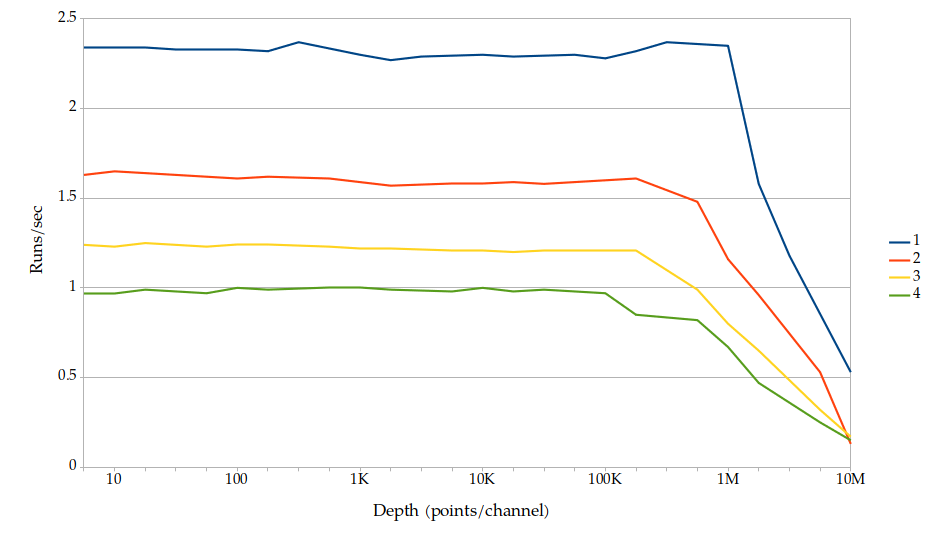
\includegraphics[width=16cm]{images/siglent-samples.png}
\caption{Siglent sample speed for various combinations of depth and channels}
\label{siglent_sample}
\end{figure}


\begin{tabularx}{16cm}{llX}
\thickhline
\textbf{Channels} & \textbf{Memory depth} & \textbf{WFM/s}\\
\thickhline
1 & 5-100K & 2.3 \\
\thinhline
2 & 5-100K & 1.6 \\
\thinhline
3 & 5-100K & 1.2 \\
\thinhline
4 & 5-100K & 1 \\
\thinhline
1 & 10M & 0.5 \\
\thinhline
2-4 & 10M & 0.15 \\
\thickhline
\end{tabularx}

These figures were obtained from a SDS2104X+ running firmware version 1.3.7R5. Different scopes and software
revisions may vary. This series of scopes support sample depths up to 100MPoints, but depths beyond 10MPoints
require a different software interface and are likely to be extremely slow, so have not yet been implemented.

\section{Teledyne LeCroy / LeCroy}

Teledyne LeCroy (and older LeCroy) devices use the same driver, but two different transports for LAN connections.

While all Teledyne LeCroy / LeCroy devices use almost identical SCPI command sets, Windows based devices running
XStream or MAUI use a custom framing protocol (``vicp") around the SCPI data while the lower end RTOS based devices use
raw SCPI over TCP (``lan").

Please see the table below for details on which configuration to use with  your hardware.

\begin{tabularx}{16cm}{lllX}
\thickhline
\textbf{Device Family} & \textbf{Driver} & \textbf{Transport} & \textbf{Notes} \\
\thickhline
DDA & lecroy & vicp & Tested on DDA5000A series \\
\thickhline
HDO & lecroy & vicp & Tested on HDO9000 series \\
\thickhline
LabMaster & lecroy & vicp & Untested, but should work\\
\thickhline
MDA & lecroy & vicp & Untested, but should work\\
\thickhline
SDA & lecroy & vicp & Tested on SDA 8Zi series\\
\thickhline
T3DSO & ??? & ??? & Untested\\
\thickhline
WaveAce & ??? & ??? & Untested\\
\thickhline
WaveJet & ??? & ??? & Untested\\
\thickhline
WaveMaster & lecroy & vicp & Untested but should be same as SDA/DDA\\
\thickhline
WaveRunner & lecroy & vicp & Tested on WaveRunner Xi and 8000 series\\
\thickhline
WaveSurfer & lecroy & vicp & Tested on WaveSurfer 3000 series \\
\thickhline
\end{tabularx}

\subsection{lecroy}

This is the primary driver for MAUI based Teledyne LeCroy / LeCroy devices.

This driver has been tested on a wide range of Teledyne LeCroy / LeCroy hardware. It should be compatible with any
Teledyne LeCroy or LeCroy oscilloscope running Windows XP or newer and the MAUI or XStream software.

\subsubsection{Typical Performance (HDO9204, VICP)}

\begin{tabularx}{16cm}{llX}
\thickhline
\textbf{Channels} & \textbf{Memory depth} & \textbf{WFM/s}\\
\thickhline
1 & 100K & >50 \\
\thinhline
1 & 400K & 29 - 35 \\
\thinhline
2 & 100K & 30 - 40 \\
\thinhline
4 & 100K & 17 - 21 \\
\thinhline
1 & 2M & 9 - 11 \\
\thinhline
1 & 10M & 2.2 - 2.6 \\
\thinhline
4 & 1M & 5.2 - 6.5 \\
\thinhline
1 & 64M & 0.41 - 0.42 \\
\thinhline
2 & 64M & 0.21 - 0.23 \\
\thinhline
4 & 64M & 0.12 - 0.13 \\
\thickhline
\end{tabularx}

\subsubsection{Typical Performance (WaveRunner 8404M-MS, VICP)}

\begin{tabularx}{16cm}{llX}
\thickhline
\textbf{Channels} & \textbf{Memory depth} & \textbf{WFM/s}\\
\thickhline
1 & 80K & 35 - 45 \\
\thinhline
2 & 80K & 35 - 45 \\
\thinhline
2 & 800K & 16 - 17 \\
\thinhline
2 & 8M & 3.1 - 3.2 \\
\thickhline
\end{tabularx}


\section{Tektronix}

This driver is being primarily developed on a MSO64. It supports SCPI over LXI VXI-11 or TCP sockets.

The hardware supports USBTMC, however waveform download via USBTMC does not work with libscopehal for unknown reasons.

\begin{tabularx}{16cm}{lllX}
\thickhline
\textbf{Device Family} & \textbf{Driver} & \textbf{Transport} & \textbf{Notes} \\
\thickhline
MSO5 series & tektronix & lan, lxi &  \\
\thickhline
MSO6 series & tektronix & lan, lxi &  \\
\thickhline
\end{tabularx}

\subsection{Note regarding ``lan" transport on MSO5/6}

The default settings for raw SCPI access on the MSO6 series use a full terminal emulator rather than raw SCPI
commands. To remove the prompts and help text, go to Utility | I/O, then under the Socket Server panel select protocol
``None" rather than the default of ``Terminal".

\subsubsection{Typical Performance (MSO64, LXI, embedded OS)}

\begin{tabularx}{16cm}{llX}
\thickhline
\textbf{Channels} & \textbf{Memory depth} & \textbf{WFM/s}\\
\thickhline
1 & 50K & 10.3 - 11.4 \\
\thinhline
2 & 50K & 6.7 - 7.2 \\
\thinhline
4 & 50K & 5.1 - 5.3 \\
\thinhline
1 & 500K & 8.7 - 9.5 \\
\thinhline
4 & 500K & 3.8 - 3.9 \\
\thickhline
\end{tabularx}

\section{Xilinx}
TODO (scopehal:40)
